\makeatletter
\def\setsize{\csname @setfontsize\endcsname \setsize}

\newcommand{\PT}{\setsize{36pt}{19pt}\bfseries} 
\newcommand{\PN}{\setsize{48pt}{50.5pt}\bfseries} 

\renewcommand\part{%
  \if@openright
    \cleardoublepage
  \else
    \clearpage
  \fi
  \thispagestyle{empty}
  \if@twocolumn
    \onecolumn
    \@tempswatrue
  \else
    \@tempswafalse
  \fi
  \secdef\@part\@spart}


  \def\@part[#1]#2{
    \begin{center}     \ifnum \c@secnumdepth >-2\relax
        \refstepcounter{part}%
        \addcontentsline{toc}{part}{\thepart\hspace{1em}#1}%
      \else
        \addcontentsline{toc}{part}{#1}%
      \fi
      \markboth{}{}%
      {
       \interlinepenalty \@M
       \normalfont
       \ifnum \c@secnumdepth >-2\relax
 \par\nobreak\vspace*{72pt}
         {\PN Part \thepart } \par\nobreak
         \vspace*{22pt}
			\ifnum\c@part=1
			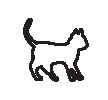
\includegraphics[width=3in]{cat}\par\nobreak
			\fi
			\ifnum\c@part=2
			\includegraphics[width=3in]{graphics/Part_2}\par\nobreak
			\fi
			\ifnum\c@part=3
			\includegraphics[width=3in]{graphics/Part_3}\par\nobreak
			\fi
         \vspace*{12pt}
           \fi
       {\PT #2}\par
       }
\end{center}
\@endpart}

\makeatother